%!TEX program = xelatex

\documentclass[11pt,titlepage]{report}
%!TEX root = main.tex

\usepackage[T1]{fontenc}
\usepackage{lmodern}
\usepackage[svgnames]{xcolor}
\usepackage{fontspec} % XeLaTeX required!
\usepackage{graphicx}
\usepackage{circuitikz}
\usepackage{tikz}
\usepackage{pifont}
\usepackage[some]{background}
\usepackage{xltxtra} 
\usepackage{setspace}
\usepackage[absolute]{textpos}
\usepackage[latin1]{inputenc}
\usepackage[english]{babel}
\usepackage{graphicx}
\usepackage{wrapfig}
\usepackage{fullpage}
\usepackage[margin=1in]{geometry}
\usepackage{float}
\usepackage{url}
\usepackage{multicol}
\usepackage{hyperref}
\usepackage{titlepic}
\usepackage{standalone}
\usepackage{siunitx}
\usepackage{booktabs}
\usepackage{amsmath}
\usepackage{unicode-math}
\usepackage{verbatim}
\usepackage{enumitem}
\usepackage{listings}
\usepackage{multirow}
\usepackage{pgfplots}
\pgfplotsset{compat=1.8}
\usepackage{caption} 
\usepackage[parfill]{parskip}
\usepackage{import}
\usepackage[backend=bibtexu,texencoding=utf8,bibencoding=utf8,style=ieee,sortlocale=en_GB,language=auto]{biblatex}
\usepackage[strict,autostyle]{csquotes}
\usepackage[final]{pdfpages}
\usepackage{subcaption}
\usepackage{ifplatform}
%\captionsetup[table]{skip=10pt}


% Fix for includepdf bug in Mac OS X
\newcommand{\insertpdfpath}[1]{
	\ifwindows
	\newcommand{\insertpdf}[2]{\includepdf[pages=##1]{##2}}
	\else
	\newcommand{\insertpdf}[2]{\includepdf[pages=##1]{#1/##2}}
	\fi
}

%set fonts
\setmainfont[Ligatures=TeX]{Myriad Pro}
\setmathfont{Asana Math}
\setmonofont{Lucida Console}

\usepackage{titlesec, color}
\renewcommand{\familydefault}{\sfdefault} %set font family
\renewcommand{\arraystretch}{1.2} %set table vertical spacing
\setlength\parindent{0pt} %no paragraph indent
\hypersetup{ %setup hyperlinks
    colorlinks,
    citecolor=black,
    filecolor=black,
    linkcolor=black,
    urlcolor=black
}

%redesign chapter headings
\definecolor{gray75}{gray}{0.75}
\newcommand{\chapternumber}{\thechapter}
\newcommand{\hsp}{\hspace{20pt}}
\titleformat{\chapter}[hang]{\Huge\bfseries}{\chapternumber\hsp\textcolor{gray75}{|}\hsp}{0pt}{\Huge\bfseries}

%Redefine appendix headers
\renewcommand{\appendixname}{Appendix}
\renewcommand{\appendixtocname}{Appendices}
\renewcommand{\appendixpagename}{Appendices}

%For code listings
\definecolor{black}{rgb}{0,0,0}
\definecolor{browntags}{rgb}{0.65,0.1,0.1}
\definecolor{bluestrings}{rgb}{0,0,1}
\definecolor{graycomments}{rgb}{0.4,0.4,0.4}
\definecolor{redkeywords}{rgb}{1,0,0}
\definecolor{bluekeywords}{rgb}{0.13,0.13,0.8}
\definecolor{greencomments}{rgb}{0,0.5,0}
\definecolor{redstrings}{rgb}{0.9,0,0}
\definecolor{purpleidentifiers}{rgb}{0.01,0,0.01}


\lstdefinestyle{csharp}{
language=[Sharp]C,
showspaces=false,
showtabs=false,
breaklines=true,
showstringspaces=false,
breakatwhitespace=true,
escapeinside={(*@}{@*)},
columns=fullflexible,
commentstyle=\color{greencomments},
keywordstyle=\color{bluekeywords}\bfseries,
stringstyle=\color{redstrings},
identifierstyle=\color{purpleidentifiers},
basicstyle=\ttfamily\small}

\lstdefinestyle{c}{
language=C,
showspaces=false,
showtabs=false,
breaklines=true,
showstringspaces=false,
breakatwhitespace=true,
escapeinside={(*@}{@*)},
columns=fullflexible,
commentstyle=\color{greencomments},
keywordstyle=\color{bluekeywords}\bfseries,
stringstyle=\color{redstrings},
identifierstyle=\color{purpleidentifiers},
}

\lstdefinestyle{matlab}{
language=Matlab,
showspaces=false,
showtabs=false,
breaklines=true,
showstringspaces=false,
breakatwhitespace=true,
escapeinside={(*@}{@*)},
columns=fullflexible,
commentstyle=\color{greencomments},
keywordstyle=\color{bluekeywords}\bfseries,
stringstyle=\color{redstrings},
identifierstyle=\color{purpleidentifiers}
}

\lstdefinestyle{vhdl}{
language=VHDL,
showspaces=false,
showtabs=false,
breaklines=true,
showstringspaces=false,
breakatwhitespace=true,
escapeinside={(*@}{@*)},
columns=fullflexible,
commentstyle=\color{greencomments},
keywordstyle=\color{bluekeywords}\bfseries,
stringstyle=\color{redstrings},
identifierstyle=\color{purpleidentifiers}
}

\lstdefinestyle{xaml}{
language=XML,
showspaces=false,
showtabs=false,
breaklines=true,
showstringspaces=false,
breakatwhitespace=true,
escapeinside={(*@}{@*)},
columns=fullflexible,
commentstyle=\color{greencomments},
keywordstyle=\color{redkeywords},
stringstyle=\color{bluestrings},
tagstyle=\color{browntags},
morestring=[b]",
  morecomment=[s]{<?}{?>},
  morekeywords={xmlns,version,typex:AsyncRecords,x:Arguments,x:Boolean,x:Byte,x:Char,x:Class,x:ClassAttributes,x:ClassModifier,x:Code,x:ConnectionId,x:Decimal,x:Double,x:FactoryMethod,x:FieldModifier,x:Int16,x:Int32,x:Int64,x:Key,x:Members,x:Name,x:Object,x:Property,x:Shared,x:Single,x:String,x:Subclass,x:SynchronousMode,x:TimeSpan,x:TypeArguments,x:Uid,x:Uri,x:XData,Grid.Column,Grid.ColumnSpan,Click,ClipToBounds,Content,DropDownOpened,FontSize,Foreground,Header,Height,HorizontalAlignment,HorizontalContentAlignment,IsCancel,IsDefault,IsEnabled,IsSelected,Margin,MinHeight,MinWidth,Padding,SnapsToDevicePixels,Target,TextWrapping,Title,VerticalAlignment,VerticalContentAlignment,Width,WindowStartupLocation,Binding,Mode,OneWay,xmlns:x}
}

\lstdefinestyle{matlab}{
language=Matlab,
showspaces=false,
showtabs=false,
breaklines=true,
showstringspaces=false,
breakatwhitespace=true,
escapeinside={(*@}{@*)},
columns=fullflexible,
commentstyle=\color{greencomments},
keywordstyle=\color{bluekeywords}\bfseries,
stringstyle=\color{purpleidentifiers},
identifierstyle=\color{purpleidentifiers}
}

%defaults
\lstset{
basicstyle=\ttfamily\small,
extendedchars=false,
numbers=left,
numberstyle=\ttfamily\tiny,
stepnumber=1,
tabsize=4,
numbersep=5pt
}
\addbibresource{../../library/bibliography.bib}

\begin{document}

\chapter{Assignment 2}
\section{Labday 4}

\subsection{Report 1}
\label{subsec:ass2-report-1}
As calculated in Section~\ref{subsec:ass1-rep-12-13} the sampling frequency should be $F_s=\SI{34}{\kilo\hertz}$ in order to obtain a \SI{1}{\centi\meter} spatial resolution. For our measurements we will use a commonly supported sampling rate of \SI{44.1}{\kilo\hertz}\footnote{See \url{http://www.cs.columbia.edu/~hgs/audio/44.1.html} for details on why \SI{44.1}{\kilo\hertz} is dominant.}. This sampling rate would then allow for a resolution of $34 / 44.1 = \SI{0.78}{\centi\meter}$. The maximum propagation delay corresponding to \SI{5}{\meter} is $t_{\text{5m}}=5/340=\SI{147}{\milli\second}$. This corresponds with \num{649} samples at \SI{44.1}{\kilo\hertz}, thus defining the peak search interval.

\begin{figure}[H]
	\centering
	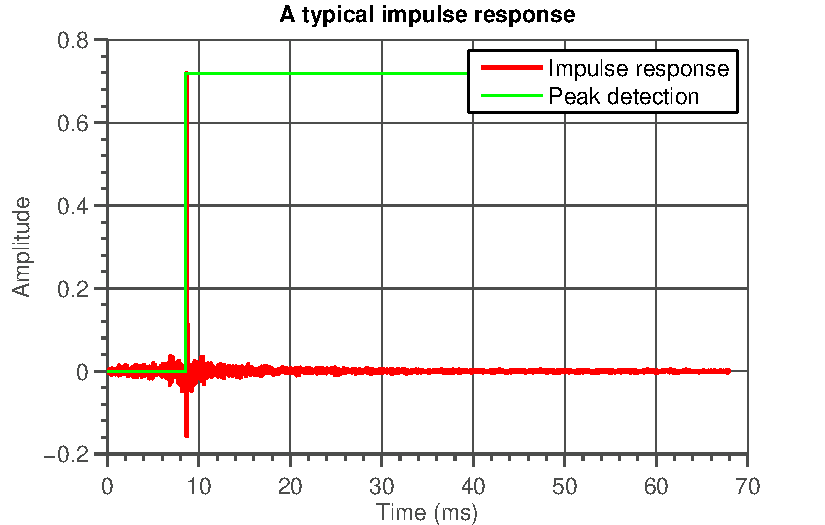
\includegraphics[width=0.8\textwidth]{../../deliverable-7-resources/figures/ass-2/report-1/ass-2-report-1.pdf}
	\caption{A typical impulse response with the detected peak.}
	\label{fig:ass-2-rep-1-typical}
\end{figure}

A typical channel impulse response is shown in figure \ref{fig:ass-2-rep-1-typical} from which we can see that a typical impulse response takes about \SI{10}{\milli\second} before it is no longer distinguishable from noise. Therefore, we chose \texttt{timer3} to be \SI{8}{\hertz} so that the repetition period is \SI{0.125}{\milli\second}.

The peak detection algorithm we designed initially used \texttt{MATLAB}'s \texttt{findpeaks} function, but it was decided to swap it for an algorithm measuring the standard deviation of small, moving intervals of the signal. The rationale is that when no peak is detected (e.g. the signal consists of only noise) the signal has a variance of $\sigma_n^2$. Then, when a peak is detected the standard deviation changes because the amplitude of the deconvolved signal changes quite suddenly. This detection algorithm seems flexible and works, as demonstrated by the green line in figure \ref{fig:ass-2-rep-1-typical}

\subsection{Report 2,3 and 4}
The TDOA algorithm that we implemented has the following basic procedure: 
\begin{enumerate}
\item Send a signal $x[n]$ through a speaker to two microphones
\item The microphones pick up signals $y_1[n]$ and $y_2[n]$
\item Calculate $h_i[n]$ from $y_i[n]=x[n]*h_i[n]$ 
\item Search for peaks in $h_i[n]$ and determine the number of samples between the peaks in $h_1[n]$ and $h_2[n]$.
\item From the number of samples in between peaks the time difference can be computed (the TDOA) and using the speed of sound the distance between the microphones.
\end{enumerate}
Note that for step three multiple methods are suitable. Three are described in the manual: deconvolution using matrix inversion, a matched filter approach and frequency domain deconvolution. For this report we decided to use the method of deconvolution using matrix inversion because initial testing yielded the best results with this method and are within arms reach because powerful computer hardware is available. %%INSERT SOURCE CODE!
\begin{figure}[H]
	\centering
	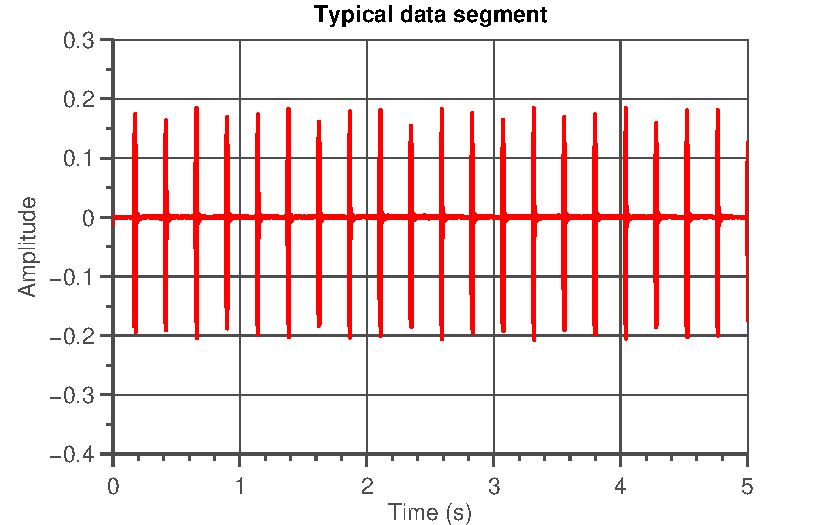
\includegraphics[width=0.8\textwidth]{../../deliverable-7-resources/figures/ass-2/report-2-3/ass-2-report-2-typical-data-segment.pdf}
	\caption{Typical received data segment.}
	\label{fig:ass-2-rep-2-data-segment}
\end{figure}

An example of a received data segment is shown in figure \ref{fig:ass-2-rep-2-data-segment}. For details on the peak detection algorithm, refer to section \ref{ass2-report-1}. For an example of the location of the peak as detected by our software see figure \ref{fig:ass-2-rep-1-typical}.

\begin{figure}[H]
	\centering
	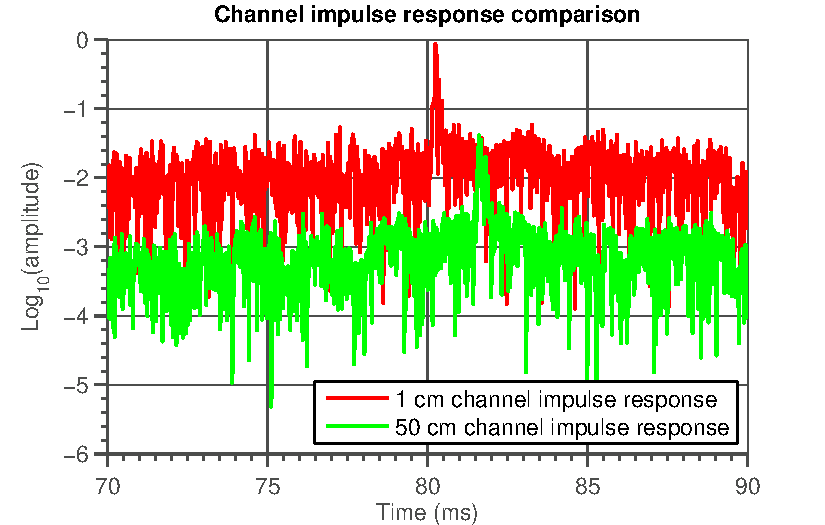
\includegraphics[width=0.8\textwidth]{../../deliverable-7-resources/figures/ass-2/report-2-3/ass-2-report-2-impulse-responses-4.pdf}
	\caption{Comparison of impulse responses for different microphone distances.}
	\label{fig:ass-2-rep-2-impulse-1-20}
\end{figure}

A response of one of our measurements is shown in figure \ref{fig:ass-2-rep-2-impulse-1-20}. This plot is a good example of two microphones placed some distance apart because it is clear the amplitudes of the two responses are about a factor two different. 

\begin{figure}[H]
	\centering
	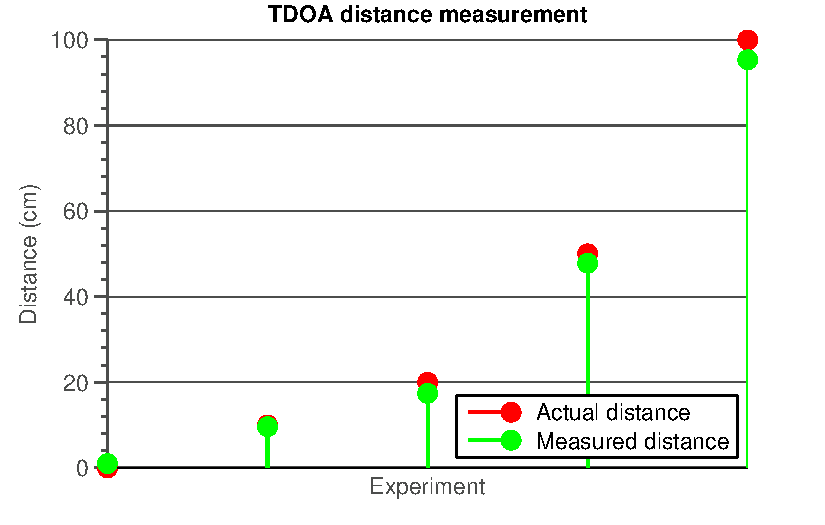
\includegraphics[width=0.8\textwidth]{../../deliverable-7-resources/figures/ass-2/report-2-3/ass-2-report-2-results.pdf}
	\caption{TDOA estimations for different microphone distances.}
	\label{fig:ass-2-rep-2-result}
\end{figure}

Figure \ref{fig:ass-2-rep-2-result} shows an overview of the TDOA distance estimations for microphones placed \num{0}, \num{10}, \num{20}, \num{50} and \SI{100}{\centi\meter}. Shown in green are the TDOA estimations and shown in red the actual distances between microphones. We can see that for larger spacing between the microphones, the estimation becomes worse. This is to be expected; when the microphones are placed further apart the signal to noise ratio at the microphone farthest away will be significantly lower than for closer placed microphones, thus making it more difficult for the peak detection algorithm to pinpoint the exact sample in which the peak occurs.

\begin{figure}[H]
	\centering
	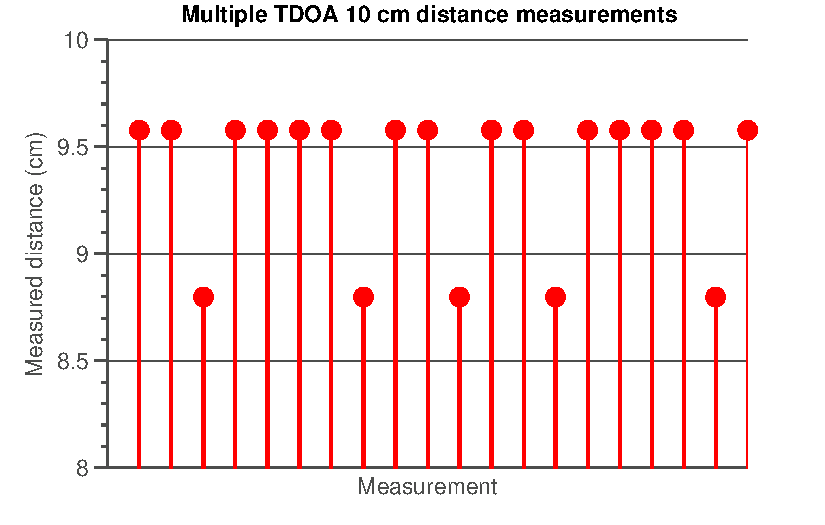
\includegraphics[width=0.8\textwidth]{../../deliverable-7-resources/figures/ass-2/report-2-3/ass-2-report-3.pdf}
	\caption{Multiple TDOA estimations for the same microphone placement.}
	\label{fig:ass-2-rep-3}
\end{figure}

An overview of multiple TDOA estimations for the same microphone placement (\SI{10}{\centi\meter} between the microphones) is shown in figure \ref{fig:ass-2-rep-3}. We calculated the average estimation to be \SI{9.38}{\centi\meter} with a standard deviation of \SI{0.35}{\centi\meter}. Because the true distance was \SI{10}{\centi\meter} we see that the measurements have a slight negative bias averaging an error of \SI{-0.62}{\centi\meter}. The measured distances are not distributed continuously, but rather discrete. This is of course due to the nature of a sampled signal; either the peak occurs at one sample or the next, there is no middle ground. From this plot we can also note the spatial resolution of the TDOA algorithm assuming the difference between the peaks at \SI{8.8}{\centi\meter} and \SI{9.6}{\centi\meter} is one  sample, the resolution is around \SI{0.8}{\centi\meter}, which corresponds perfectly to the value calculated in Section~\ref{subsec:ass2-report-1}.

\subsection{Report 5}
The general idea of the deconvolution approach is that a signal $y[n]=x[n]*h[n]$ is received, where $h[n]$ is the channel response. The deconvolution method using matrix inversion tells us the channel can be approximated by $\hat{h}=(\mat{X}^T\mat{X})^{-1}\mat{X}^T\vec{y}$. Because the sent signal $x[n]$ is known, the matrix $\mat{X}^\dagger=(\mat{X}^T\mat{X})^{-1}\mat{X}^T$ can be pre-computed, leaving only a matrix multiplication every time $\hat{h}$ must be computed. 

In the method outlined above it is immediately clear that for the same (or similar) $\mat{X}^\dagger$ matrices (and thus $x[n]$ codes) the channel estimation will produce incorrect results. While mathematically not correct, it can be intuitively thought of as follows: the algorithm looks for $x_1[n]$ occurring in $y[n]$. Now if we have a second $x$, $x_2[n]$ and this $x_2[n]$ is similar to $x_1[n]$ then it can be expected that the algorithm mistakes an occurrence of $x_1[n]$ for an occurrence of $x_2[n]$. More mathematically, we want the detected channel impuse $\hat{h}$ to have a strong cross-correlation with the sent signal $x_1[n]$ and little cross-correlation with any other signal. This last requirement can be achieved by choosing a signal that covers a broad spectrum (i.e. is generated pseudo-randomly) and is of sufficient length.
%VOLGENS MIJ IS HET VOLGENDE NIET VERSLAGWAARDIG!
%\subsection{5-channel TCOA measurements}
%Read page 106 for more info
\end{document}